
Because of the necessity to approximate the exchange-correlation energy $E_{xc}[\rho(\bm{r})]$ as a functional of single-electron density $\rho(\bm{r})$,  there are challenging cases where DFAs failed to determine the energetics of molecular and material systems quantitatively or even qualitatively.\cite{cohen2012challenges} In particular, the delocalisation error is regarded as the most outstanding challenge in the developments of DFAs,\cite{bryenton2023delocalization} which is most relevant to the \textit{band gap problem}\cite{perdew1985density} in the community of materials modelling. The semilocal nature of $E_{xc}[\rho(\bm{r})]$ also leads to the failure in determining the correct (equilibrium) structures and interaction energies of systems that are bounded by the (non-covalent) dispersion interactions. Fortunately, many robust and  efficient theoretical approaches have been developed to correct such a deficiency in standard DFAs.\cite{grimme2016dispersion} Here, we aim to provide some concise and explanatory accounts on these two challenges for readers  who are  interested in applying DFT solving problems in real material designs and discoveries to become aware of the limitations in the underlying methodologies applied in their research. For readers who are more interested in   different theoretical aspects and the latest developments behind DFT, we refer them to this interesting article\cite{DFT_exchange} that exchanges  viewpoints on DFT by the leading theoreticians in the research community.

\paragraph{\textbf{The delocalisation error}} The delocalisation error is a term that expands\cite{perdew1982density,ruzsinszky2006spurious,mori2006many} on the originally coined self-interaction error (SIE)\cite{perdew1981self}  to cover more general context in DFT. \citet{hait2018delocalization} have provided a good explanation on the relationship between these two terms, which will be quoted here (in \emph{italics}). The delocalisation error originates in defining the electrostatic repulsion term $E_{J}=\frac{1}{2}\iint \frac{\rho(\bm{r})\rho(\bm{r}^\prime)}{\left\vert \bm{r}-\bm{r}^\prime\right\vert}d\bm{r}d\bm{r}^\prime$ [\cref{eq:KS_eqn}] based on the one-particle electron density. \emph{However, $\rho(\bm{r})$ is made up of discrete number of electrons, which (despite being delocalised over space) should not be able to interact with themselves. $E_J$ therefore contains a spurious self-repulsion energy. The exchange-correlation energy }($E_{xc}[\rho(\bm{r})]$) \emph{in principle should fix this, but the correction is very approximate for most functionals on account of the $E_{xc}$ functional having substantial local components, while self-repulsion is explicitly non-local. The electron density subsequently delocalises (becomes less compact) in order to minimise the residual self-repulsion}, resulting in the delocalisation error.

\begin{figure}[tb]
    \centering
    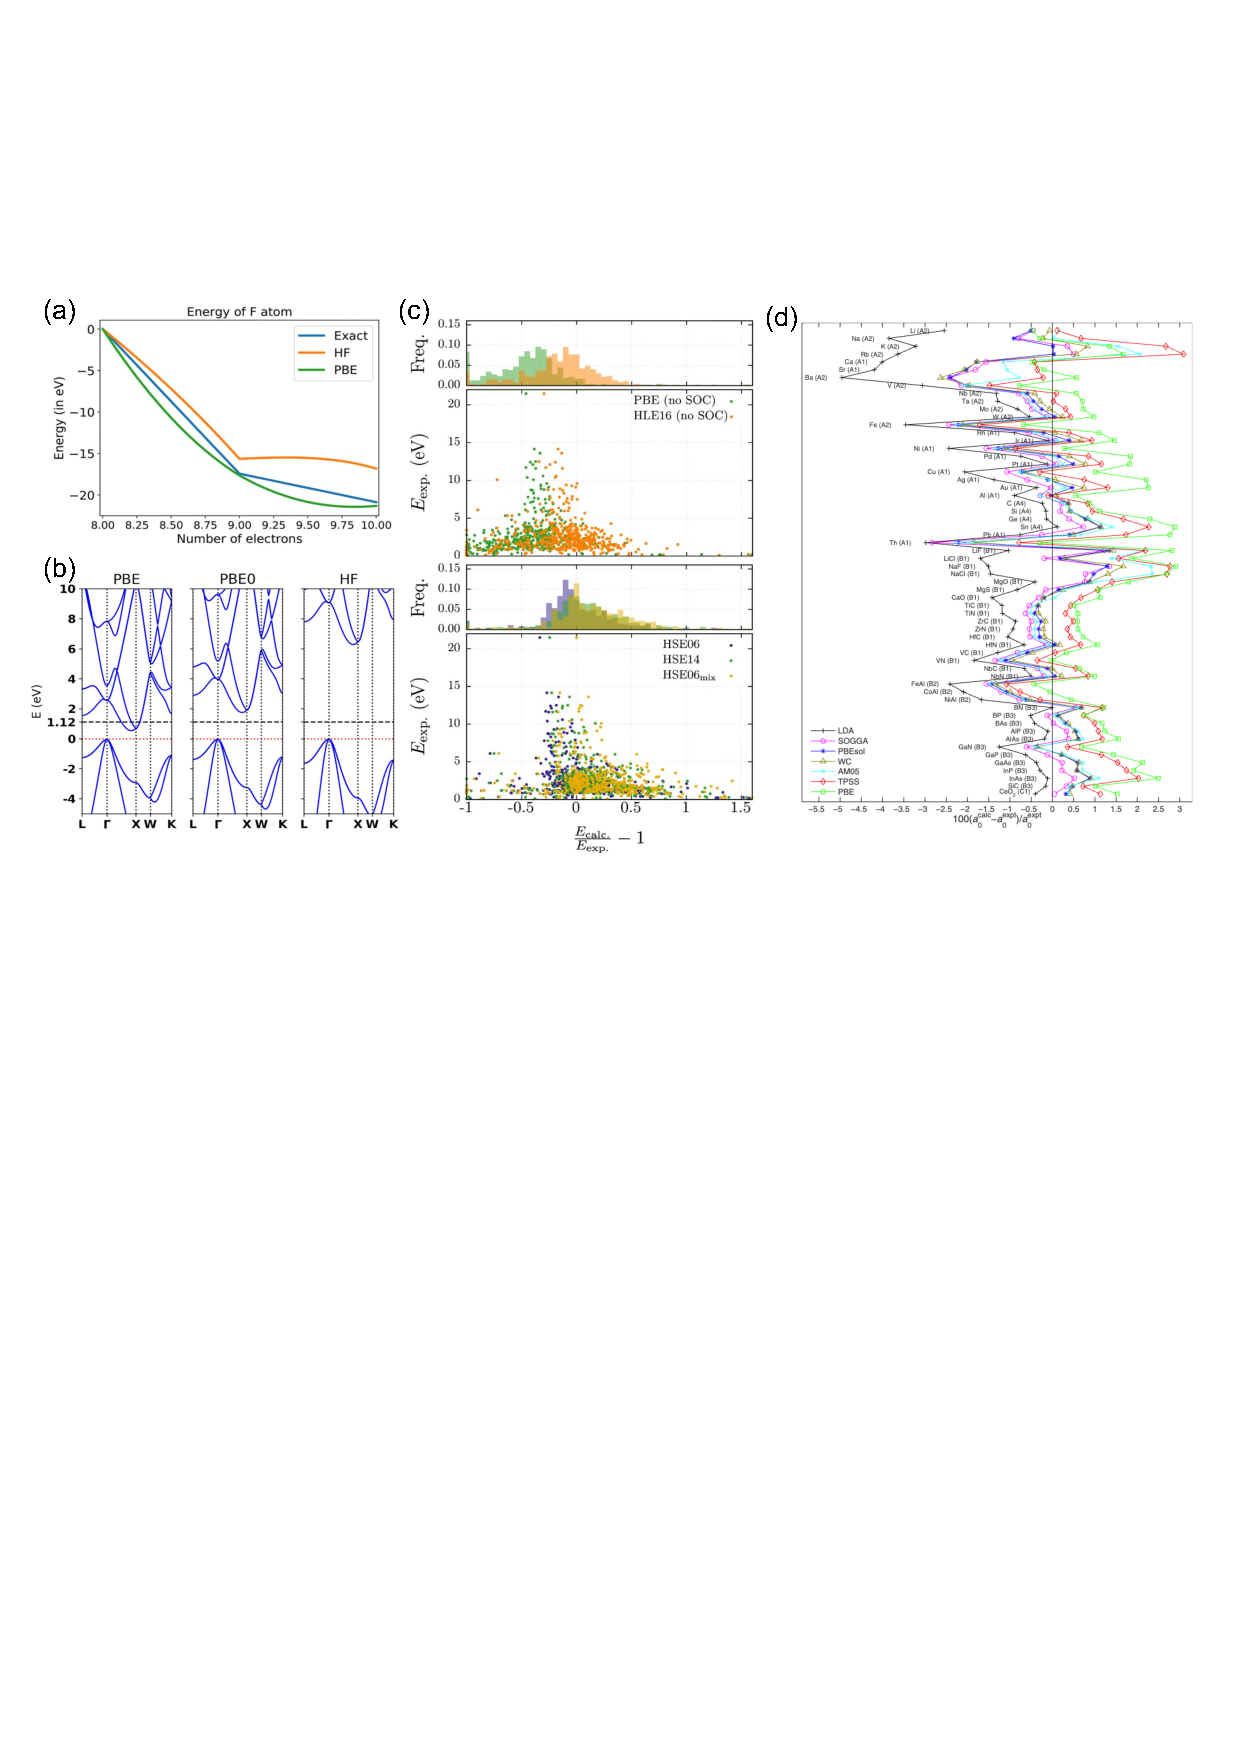
\includegraphics[width=\linewidth]{DFT_bandgaps.pdf}
    \caption{Fractional charges and the band gap problems in DFT. (a) Effect of delocalisation error on fractional charges, showing the overestimation of energy by HF and underestimation by a typical GGA functional (PBE) [from \citet{hait2018delocalization}]. (b) Variations in the computed electronic band structures for bulk silicon, showing strong dependence on the content of exact HF exchange (PBE: 0\%, PBE0: 25\% and HF: 100\%) ,ixing in the exchange-correlation functionals [from \citet{bryenton2023delocalization}
]. (c) Benchmarking the performances of different DFAs in predicting the band gaps for 472 non-magnetic materials. The figures shows the relative frequency and experimental band gap ($E_{\mbox{\scriptsize{exp.}}}$) as a function of the ratio between theoretical ($E_{\mbox{\scriptsize{calc.}}}$) and experimental band gaps for the different exchange-correlational functionals [from \citet{borlido2019large}].  To compare the performance of GGA functionals in reproducing the structural properties of solids, in (d), we also show the relative error  in the calculated lattice constants for selected inorganic solids with respect to the experimental data. Overall, the PBEsol functional gives the lowest mean absolute relative error of 9.5\% compared to all other functionals tested.  [from \citet{haas2009calculation}] }
    \label{fig:DFT_bandgap}
\end{figure}

In their review, \citet{bryenton2023delocalization} summarised a few different images that can be applied to interpret the origins of, and consequences resulting from the SIE in predicting the properties of molecular and material systems using DFT. Here, we focus on the \emph{fractional charge} picture, which is best suitable for explaining the well-known \emph{band gap problem} in DFT, particularly for strongly correlated systems and Mott insulators,\cite{cohen2012challenges} that is most relevant to the field of theory-driven material designs.

In this seminal work, \citet{perdew1982density} shows that the total energy of a multielectron system containing a fractional number of electrons $N+\omega$ [$N\in \mathbb{Z}$ and $\omega \in (0,1)$] should be $E(N+\omega)=(1-\omega)N(E)+\omega E(N+1)$, which is a straight line that interpolates between the total energies of two systems containing $N$ and $N+1$ electrons, respectively, with discontinuities at the integer numbers of electrons. However, as semilocal DFAs (such as PBE) tend to stabilises the delocalised electron densities, they generate states with fractional charges that are lower in energies than what is expected from the linear interpolation [\cref{fig:DFT_bandgap}(a)]. A more concrete example is to consider the H$_{2}^{+}$ ion at its dissociation limit, which, instead of producing the correct configuration of H$^{+}\cdots$H, with the charge localised predominantly on one hydrogen ion, most DFAs will stablise the complex  H$^{\delta +}\cdots$H$^{\delta +}$ with fractional charges equally distributed on both ions. It should also be noted that, the energy curve $E(N+\omega)$ corresponding to HF shows a concave-down behaviour [\cref{fig:DFT_bandgap}(a)], indicating its tendency to produce more localised electron densities.

The challenge behind standard DFAs in correctly predicting the electronic band gap could be understood from their molecular equivalent of the HOMO-LUMO gap, which \citet{janak1978proof} first showed that the orbital eigenenergies are the left- and right-derivatives with respect to the electron number,
\begin{equation}\label{eq:HOMO_LUMO_def}
\varepsilon^{\mbox{\scriptsize{HOMO}}}=\lim_{x\to N^{-}}\frac{E(x)-E(N)}{x-N},\qquad \varepsilon^{\mbox{\scriptsize{LUMO}}}=\lim_{x\to N^{+}}\frac{E(x)-E(N)}{x-N}.
\end{equation}
As shown in \cref{fig:DFT_bandgap}(a), the `concave-up' behaviour in the $E(N)$ curve for semilocal GGA functional, it leads to $\varepsilon^{\mbox{\scriptsize{HOMO}}}$ becomes too high whereas $\varepsilon^{\mbox{\scriptsize{LOMO}}}$
becomes too low, resulting in the underestimation of the HOMO-LUMO gap, or the band gap for solids [see \cref{fig:DFT_bandgap}(b) for the illustration of the band structures for silicon]. On the other hand, it can be seen that the opposite behaviour in the $E(N)$ curve for HF resulted in a drastic overestimation of the band gap. This can be used to understand why, by including 25 \% of HF exchange into the functional PBE (PBE0),\cite{adamo1999toward} the problem of band gap underestimation by pure-GGA can be alleviated by opening up the estimated band gap values.

Putting the arguments above into a broader context, \cref{fig:DFT_bandgap}(c) shows a large-scale benchmark of the exchange-correlation functionals in calculating band gaps for 472 non-magnetic solids against their experimental values. Using the metric $\eta=E_{\mbox{\scriptsize{calc.}}}/E_{\mbox{\scriptsize{exp.}}}-1$ to compare the magnitudes of the calculated ($E_{\mbox{\scriptsize{calc.}}}$) versus experimental $(E_{\mbox{\scriptsize{exp.}}})$, \citet{borlido2019large} shows that statistically LDAs underestimate $(E_{\mbox{\scriptsize{exp.}}})$ by 50 \% while GGAs underestimate $E_{\mbox{\scriptsize{exp.}}}$ by 40 \%. Meta-GGA functionals, such as SCAN\cite{sun2013semilocal} and mBJ (modified Becke-Johnson potential)\cite{becke2006simple,tran2009accurate} show improvements from LDA/GGA results with $\sim$37 \% underestimation of  $E_{\mbox{\scriptsize{exp.}}}$. The range-separated hybrid HSE06\cite{krukau2006influence} gives the smallest mean absolute error of 0.53 eV, particularly for small band gap materials, the mean percentage error in estimating the band gap is $\sim$ 31 \%. However, the high computational costs associated with hybrid functionals generally prohibit them from being applied in studying exotic electronic properties of materials where a large number of band gap calculations are required, such as electronic dephasing in photo-absorbing semiconductors originating from the strong electron-phonon coupling in the material.\cite{li2018time,li2019anharmonicity,yang2020correlating} 

Another important consequence of the delocalisation error in DFT is the challenge to correctly determine the energetics of the charge-transfer complexes when DFT is used for predicting the properties of materials. Here, we focus on the calculation of the charge transfer integral $J_{ij}$, an important parameter in molecular electronics that is the energy required for an electron/hole to be transferred from one monomer to another in a non-covalently bounded molecular dimer [\emph{c.f.} \cref{Markus}], which is equivalent to the reaction energy of D$^{-}$+A$\to$D+A$^{-}$ (for electron transfer where D stands for donor and A for acceptor). Due to the presence of delocalisation error, standard DFT cannot be applied to determine the reaction energy since it fails to localise an extra charge on either the donor or acceptor. Methods such as the constrained density functional theory (CDFT)\cite{wu2006extracting} and frozen density embedding (FDE)\cite{pavanello2011modelling} are some of the proposed solutions to this problem, however, it still requires the careful choice of appropriate DFA to reach the right answer. For example, \citet{kubas2014electronic} put forward a benchmark set of $J_{ij}$ for 11 small molecule homodimers, which shows that PBE+50\% HF exchange gives the best result ($\sim 0.8$ \% error), whereas overestimates $J_{ij}$ by 38.7 \% because of the overly diffused charge densities produced by the pure PBE functional. In the context of energy landscape, recent study from \citet{leblanc2018pervasive} showed that, standard dispersion-corrected DFT methods failed to correctly determine the relative energetic stabilities of the proton-transferred acid-base forms of multicomponent molecular crystals over their co-crystal forms, which poses challenges in applying organic crystal structure prediction methods\cite{reilly2016report,Hunnisett:aw5093,Hunnisett:aw5094} for polymorph screenings with computationally efficient methods based on electronic structure theory. 


\paragraph{\textbf{Dispersion interactions in non-covalently bounded systems.}} Dispersion interaction is the attractive part of the vdW interaction in non-covalently bounded complexes. Being able to correctly determine the magnitudes of dispersion interactions is critical across a wide range of atomistic modellings with broad implications, including chemical reactions, catalysts, molecular recognitions, protein folding, gas adsorptions, and 2D materials. However, interaction energies determined from semilocal DFAs are generally too repulsive thus fail to give the correct binding curves of vdW complexes [\cref{fig:Ar_dimer_PES}]. This failure arises because the dispersion interaction is essentially a long-range dynamical electron correlation effect, whereby the electron densities on two interacting bodies A and B are constantly fluctuating, which generate instantaneous dipole moment on each body that attracts each other via Coulomb interaction. From the perspective of MP2 (second-order M\o{}ller–Plesset perturbation) theory,\cite{moller1934note} this correlation energy is related to the interaction energies of electrons transit from the ground to the excited states on the two interacting bodies:
\begin{equation}\label{MP2_corr}
    E_{\mbox{\scriptsize{corr}}}^{AB}=-\sum_{ia}\sum_{jb}\frac{(ia\vert jb)[(ia\vert jb)-(ib|ja)]}{\varepsilon_{a}+\varepsilon_{b}-\varepsilon_{i}-\varepsilon_{j}},
\end{equation}
in which $(ia\vert jb)=\iint \phi_i^\dagger (\bm{r}_{1})\phi_a(\bm{r}_1)\frac{1}{|\bm{r}_{1}-\bm{r}_2|} \phi_j^\dagger (\bm{r}_{2})\phi_b(\bm{r}_1)  d\bm{r}_1 d\bm{r}_2$ is the two electron integral for the particle-hole excitations involving the excitation of electron from occupied orbital $i$ (or $j$) to the unoccupied orbital $a$ (or $b$) that are localised on A (or B), with $\varepsilon$ being the corresponding orbital energy. It is therefore clear that, the involvement of excited states (contrary to DFAs which are build upon the ground state electron densities), as well as long-range electron-electron interactions (whereas DFAs are local in $\bm{r}$), make it challenge for standard DFAs to quantitatively, or even qualitatively, determines the strengths of the dispersion interactions in atomistic modelling.

\begin{figure}[tb]
    \centering
    \includegraphics[width=0.7\linewidth]{Ar_dimer_PES.png}
    \caption{Computed potential energy curves for two interacting Ar atoms with and without dispersion correction with respect to an accurate reference [Adapted from \citet{grimme2016dispersion}].}
    \label{fig:Ar_dimer_PES}
\end{figure}

In empirical atom-atom forcefields, the dispersion interaction can be modelled as $E_{\mbox{\scriptsize{disp}}}=\sum_{i<j}-C_6/R^6_{ij}$ (with the possibilities to include higher order terms such as $-C_8/R^8$ and $-C_{10}/R^{10}$) with $R_{ij}$ being the interatomic distance between atom $i$ and $j$. Modern \emph{dispersion-corrected DFAs}\cite{grimme2016dispersion} primarily builds upon this idea and correct the DFA interaction energy between two bodies A and B as $E_{\mbox{\scriptsize{tot}}}^{\mbox{\scriptsize{AB}}}=E_{\mbox{\scriptsize{DFA}}}^{\mbox{\scriptsize{AB}}}+E_{\mbox{\scriptsize{disp}}}^{\mbox{\scriptsize{AB}}}$ where $E_{\mbox{\scriptsize{disp}}}^{\mbox{\scriptsize{AB}}}$ takes the same atom pairwise form as in the empirical atom-atom forcefields, with atom-atom dispersion coefficients $C_{n}$ $(n=6,8,10\ldots)$ determined from high-level quantum chemical calculations, thus minimising the level of empiricism in the overall method. This is fundamentally possible, for example, by starting from the MP2 correlation energy [\cref{MP2_corr}], the $C_6$ coefficient is related to the frequency-dependent  polarisability $(\alpha)$ of the interacting atomic dipoles as the Casimir-Polder integral\cite{casimir1948influence} 
\begin{equation}\label{eq:casimir_eq}
    C_6^{\mbox{\scriptsize{AB}}}=\frac{3}{\pi}\int_{0}^{\infty} \alpha_{\mbox{\scriptsize{A}}}(i\omega)\alpha_{\mbox{\scriptsize{B}}}(i\omega)\mbox{d}\omega,
\end{equation}
where $\alpha$ can be calculated from time-dependent density functional theory. \cref{eq:casimir_eq} also implies that atom with lower coordination number (CN) in the structure will have a more diffused electron density, thus becomes more polarisable resulting in a larger $C_6$ coefficient. This geometry-dependent attenuation effect of dispersion coefficients is built into the major modern dispersion correction approaches to enhance the accuracy, where in the following, we will briefly review the key features of some dispersion correction schemes that are mostly used in the materials modelling community. 
